\chapter{Introduction}
Radiology is a powerful tool to detect and diagnose abnormalities by allowing doctors to visually inspect internal pathology that could not otherwise be seen. Though it is an indispensable part of the diagnostic workup, the practice of radiology is still fraught with error due to the inherently subjective nature of the task; the doctor must still visually scan, detect, and interpret the findings in the image to deliver an impression. An unfortunate consequence of such a system is substantial variability in practice and performance. This dissertation aims to tackle these shortcomings. To do so, I propose a novel computational decision-support paradigm aimed at improving the quality and content of the radiological \emph{report} rather than the traditional approaches aimed at directly improving the diagnosis. I develop informatics methods within this paradigm to detect and reduce error in reports, and show how these methods have the potential to improve overall diagnostic performance. This chapter provides an overview of the dissertation. I begin by providing a brief background of radiological error, decision-support systems, and reporting. I then give a high-level description of my proposed decision-support model, methods, and key results. Finally, I delineate my contributions to the field and provide a guide to the reader for the remainder of the document.



\section*{Radiology, variability, and errors}
Radiology is an essential part of modern clinical medicine, constituting 10.6\% of health care spending and is virtually ubiquitous in every part of health care \cite{Dodoo:tg}. The field has traditionally been at the forefront of medical technology by virtue of its foundations and reliance upon sophisticated technological achievements. Digital radiology and picture archiving and communications systems led to an early, widespread adoption of electronic records with respect to imaging \cite{Strickland:2000cv,Bryan:1999kn}. But, despite the early adoption of computational systems to manage data, the actual practice of radiology remains a relatively unchanged. An unfortunate consequence of such a system is substantial variability in practice and performance \cite{Fitzgerald:2001hn}. \citeA{Robinson:1997uq} went so far as to state that ``errors and variations in interpretation now represent the weakest aspect of clinical imaging'' and declared such issues as ``Radiology's Achilles' heel''. This is not to say that radiologists are the only doctors faced with these issues, as the now infamous Institute of Medicine report \emph{To Err is Human: Building a Safer Health System} revealed a striking amount of poor patient outcomes are a result of medical error \cite{Anonymous:2000va}. A prominent recommendation from this study is the use of automation and computation to improve upon standard of care via decision support systems.

\section*{Radiological decision-support}
Decision support systems are tools that incorporate medical information to provide meaningful input to medical practitioners. The main source of medical information in radiology is confined to patient history drawn from the electronic medical record, the patient images, and the reports generated by the radiologists. As a result, it is a ripe domain for decision support tools to assist in organizing, analyzing, and synthesizing these data sources. 

Radiological data mining allows clinicians to query similar cases to the ones they are evaluating \cite{Shin:2015wl,Bozkurt:2014jw,Depeursinge:2012ce,Korenblum:2011gx,Akgul:2011ey,Nassif:2009du}. Computer-aided detection (CADe) systems assist in identifying abnormalities in images across a variety of radiological domains such as mammography, colonoscopy, lung screening, and liver diagnosis \cite{Cheng:2003ig,Castellino:2005ke,Meeuwis:2010bv,Oliver:2010fm,Fenton:2011fw,Fenton:2012kz,Jamieson:2012hz,Gallas:2012eg,Giger:2013jb}. Computer-aided diagnosis (CADx) systems assist in interpretation of abnormalities found in the image \cite{Jiang:1999fj,ElizabethS:2005gc,Gallas:2012eg,Bright:2012ga,Giger:2013jb,Depeursinge:2010jl,Fujita:2008it,Eadie:2011cv,Rubin:2005jg,Garg:2005cb,Elter:2009fv,Jamieson:2010vl,Jamieson:2010tt,Cheng:2003ig,Jiang:2001fy} as well as interpretation of the content within the radiology report \cite{Burnside:2000wl,ElizabethS:2005gc,Burnside:2009br,Rubin:2005jg}.

Despite significant technological achievements, adoption of these systems in radiology is limited. In particular, the only commercially deployed radiological decision support systems are computer-aided detection (CADe). The main reasons for this inability to affect practice is that these systems often interrupt clinical  work-flow, give assessments rather than recommendations, and fail to provide decision-support during decision-making \cite{Kawamoto:2005gn,Morgan:2011ct}. These shortcomings are not unique to radiological decision support; they exhibit the same symptoms of decision support systems in other clinical domains that did not see commercial adoption. In general, they still follow the the so-called \emph{Greek Oracle} model of decision support \cite{Miller:1990wg,Miller:1994cx}. Such systems fail when deployed in practice since they are based on the implicit assumption that computers can perform the duties of doctors better than doctors themselves. Charles Friedman goes so far as to declare that the \emph{Fundamental Theorem of Biomedical Informatics} is that decision support should ``augment human reasoning'' beyond the capabilities of an unaided practitioner \cite{Friedman:2009dx}. Thus, it is crucial to develop radiological decision support tools that fit into the work-flow and augment their reasoning. A perfect window to provide this is during radiological reporting \cite{Noumeir:2006cb}.

\section*{Radiology reporting}
The report is of crucial importance, since it conveys the radiologist findings, interpretation of those findings, and suggested patient management. It is frequently the primary form of communication between radiologists and referring clinicians or patients \cite{Sistrom:2005cx}. Improvement of reporting directly improves such communication and indirectly may improve the radiologist's own performance. Prior studies have shown the importance of good reporting practices and identified several key traits of good reports: correctness of findings, completeness of the description of significant clinical findings, consistency of report language and findings, and timeliness of the report's completion \cite{Johnson:2004kh, HaraldO:2004hi}.

Considerable effort has been made to improve upon the variability in report content and diagnosis; arguably the most successful of which is in mammography \cite{Langlotz:2009fn,Burnside:2009ki}. The Breast Imaging-Reporting and Data System (BI-RADS) provides a standard lexicon of descriptors for radiological observations \cite{Liberman:ws}. This standardized language has virtually eliminated ambiguity in terminology across the United States. Further work has been done to create the RadLex ontology for a more universal solution to radiological terminology \cite{Langlotz:2006jn}. Yet, there is still a substantial body of work revealing variability with regard to sensitivity and specificity of evaluation of lesion malignancy amongst different readers as well as different facilities \cite{Jackson:2009fw, Beam:1996ui, Elmore:2002vc, Taplin:2008bv}. Such variability is not restricted to diagnosis and impressions; even the \emph{findings} within the contents of the report have shown variability \cite{Hobby:2000th, Robinson:1997uq}.

Another solution to improving upon radiological reports is the use of \emph{Structured Reporting Systems}. Such systems provide templates with standardized information and structure as well as support for terminologies like RadLex or BI-RADS \cite{Reiner:2009ib}. Unfortunately, structured reporting is not without its drawbacks. It is generally more time-intensive and imposes distractions in the traditional radiological workflow, directly interfering with timeliness \cite{Weiss:2008er}.

\section*{Improving performance by improving reports}
Both standardized terminology and structured reports are solid steps to improving upon the reporting process, but they do not directly analyze the radiological concepts being communicated. Borrowing from the \emph{meaning triangle}, the tools described encode radiological objects with standard expressions, but they do not encode their sense or concept. Such work would need to perform higher order analysis of the information in the report including, but not limited to, analyzing if the contents in the reports is correct, complete, or even consistent with diagnosis. In this sense, decision support systems provide the missing piece for this analysis.

Our hypothesis is that improving the correctness, consistency, and completeness of radiology reports can improve the sensitivity and specificity of diagnosis and thereby improve the quality of patient care. To tackle this challenge and to enable translation of decision-support system into clinical practice to benefit patient care, we propose a real-time decision-support system that provides feedback to radiologists as they generate their reports. This system will create evaluate and improve upon the content of a structured radiological report. This differs from traditional approaches to decision-support system because our system will improve upon reporting, and by our hypothesis, implicitly improve upon practice. By ensuring that the relevant observations are correctly, completely, and consistently described in mammography reports, our decision-support system will reduce variability in practice, improving practitioner decision making and lead to better patient care.

\section*{FASR: Fast Adaptive Structured Reporting}
The Fast Adaptive Structured Reporting (FASR) system's goal is to reduce variability and error in radiological interpretation by providing decision-support during reporting time. This works by incorporating multiple checks during the reporting process and providing real-time feedback to the radiologist.

\subsection{Specific aims}
There are three main components to FASR: (1) Verification of the annotation correctness, (2) assessment of report completeness, and (3) providing feedback to the radiologist.

\begin{figure}[h]
	\centering
	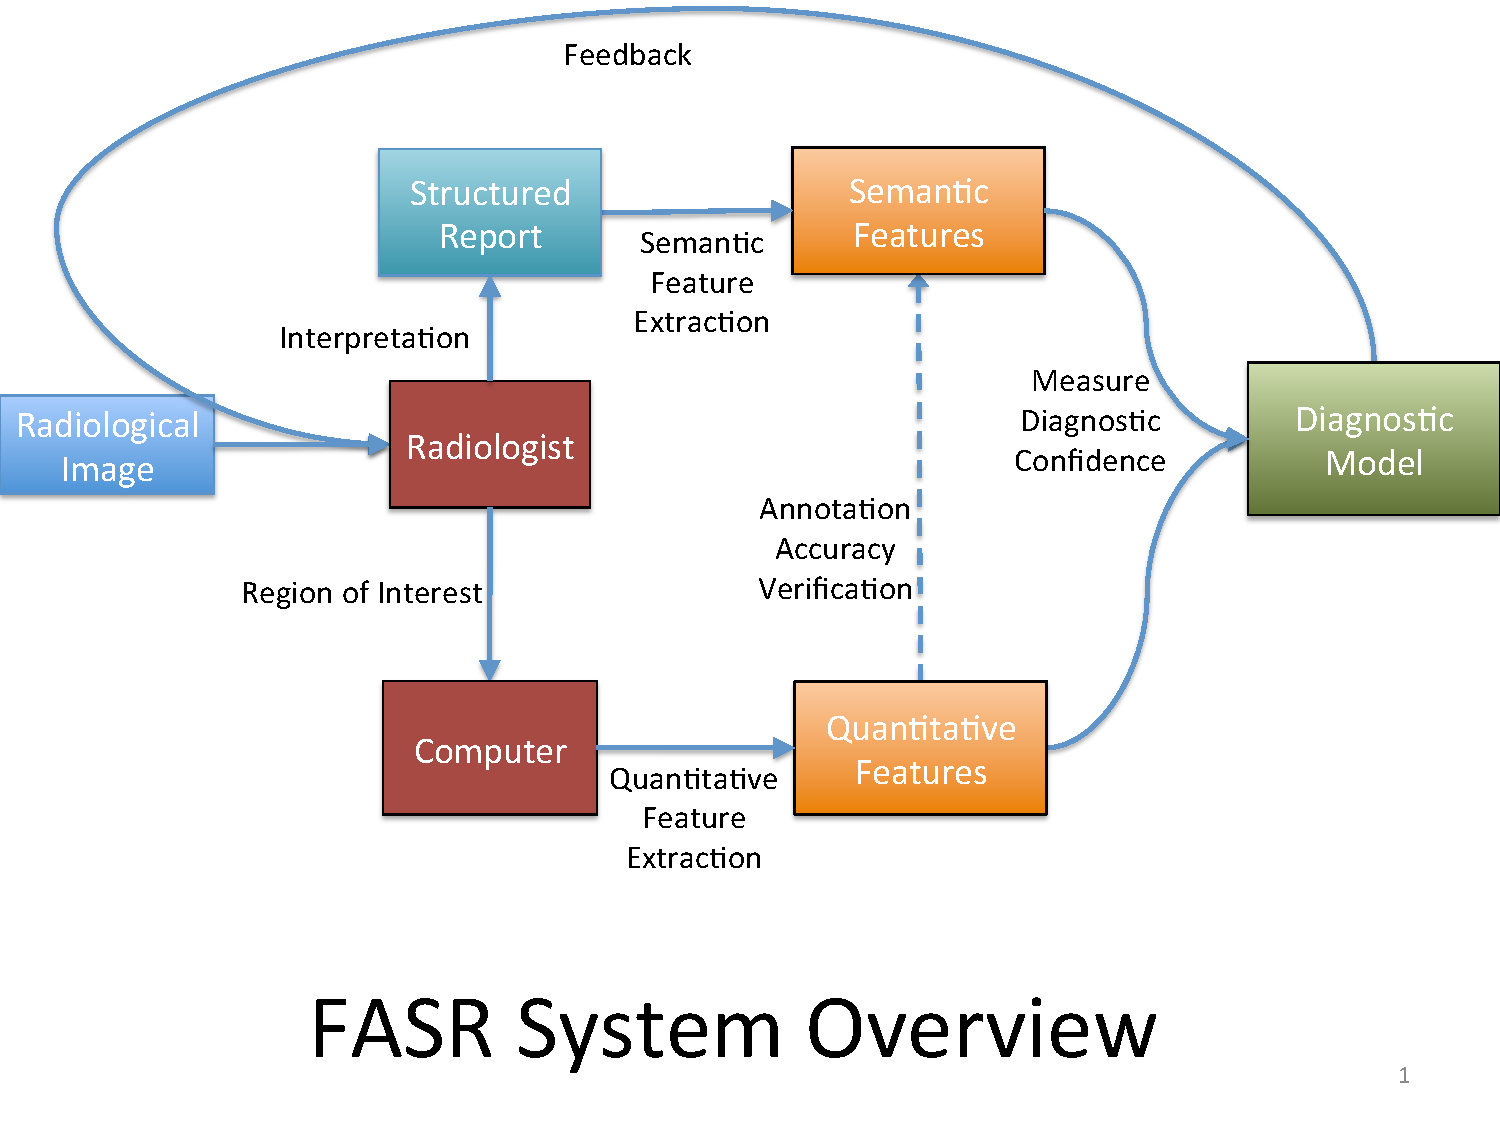
\includegraphics[width=1\linewidth]{fasr_diagram.pdf}
	\caption{Overview of the Fast Adaptive Structured Reporting (FASR) system}
	\label{fig:fasr_diagram}
\end{figure}

\subsection{Methodology}

\subsection{Key Results}


\section{Summary of contributions}
This work demonstrates contributions to the our understanding of reporting in radiology as well as performance of decision-support systems for diagnostics.

\subsection{Radiology contributions}
\subsubsection{Automatic annotation and verification of descriptors in liver CT scans}
\subsubsection{Correlated incomplete reports with diagnostic error}

\subsection{Informatics Contributions}
\subsubsection{General purpose semantic classification of images}
\subsubsection{Monte-Carlo computation of same-decision probability}
\subsubsection{Framework for delivering and evaluating feedback in decision-support systems}


\section{Guide for the reader}
